\documentclass[lang=cn,11pt,a4paper,cite=authoryear,twocolumn]{elegantpaper}

% 微分号
\newcommand{\dd}[1]{\mathrm{d}#1}
\newcommand{\pp}[1]{\partial{}#1}

\newcommand{\homep}[1]{\textbf{Problem #1}}
\newcommand{\subhomep}[1]{\textbf{SubProblem #1}}

% FT LT ZT
\newcommand{\ft}[1]{\mathscr{F}[#1]}
\newcommand{\fta}{\xrightarrow{\mathscr{F}}}
\newcommand{\lt}[1]{\mathscr{L}[#1]}
\newcommand{\lta}{\xrightarrow{\mathscr{L}}}
\newcommand{\zt}[1]{\mathscr{Z}[#1]}
\newcommand{\zta}{\xrightarrow{\mathscr{Z}}}

% 积分求和号

\newcommand{\dsum}{\displaystyle\sum}
\newcommand{\aint}{\int_{-\infty}^{+\infty}}

% 简易图片插入
\newcommand{\qfig}[3][nolabel]{
  \begin{figure}[!htb]
      \centering
      \includegraphics[width=0.4\textwidth]{#2}
      \caption{#3}
      \label{#1}
  \end{figure}
}

% 表格
\renewcommand\arraystretch{1.5}


% 日期


\title{数字电路基础\quad 第十二周作业}
\author{范云潜 18373486}
\institute{微电子学院 184111 班}
\date{\zhtoday}

\begin{document}

\maketitle

作业内容:8.2,8.5

\homep{8.2}

\(Y_1 = (B' A + B A' + C D ) ' \) 

\(Y_2 = (C D' + C' D) A B + Z (AB)' \) 

\homep{8.5}

驱动:

\(Q_0\) 的驱动: \(Q_1' Q_3 + Q_2 Q_3\) 

\(Q_1\) 的驱动: \(Q_0\) 

\(Q_2\) 的驱动: \(Q_1\) 

\(Q_3\) 的驱动: \(Q_2\) 

状态:

\(Q_0 {} _{n}  = Q_1' Q_3 + Q_2 Q_3\) 

\(Q_1 {} _{n}  = Q_0\) 

\(Q_2 {} _{n}  = Q_1\) 

\(Q_3 {} _{n}  = Q_2\) 

输出:

\(Y = Q_0 + Q_1 + Q_2 + Q_3\) 

状态图(按照1的个数排序):

\begin{lstlisting}
0000->0000

0001->0010
0010->0100
0100->1000
1000->0001

0011->0110
0110->1100
1100->1001
1001->0011

0101->1010
1010->0100

0111->1110
1110->1101
1101->1011
1011->0110

1111->1111
\end{lstlisting}

% \qfig{}{状态图}
\begin{figure}[!htb]
    \centering
    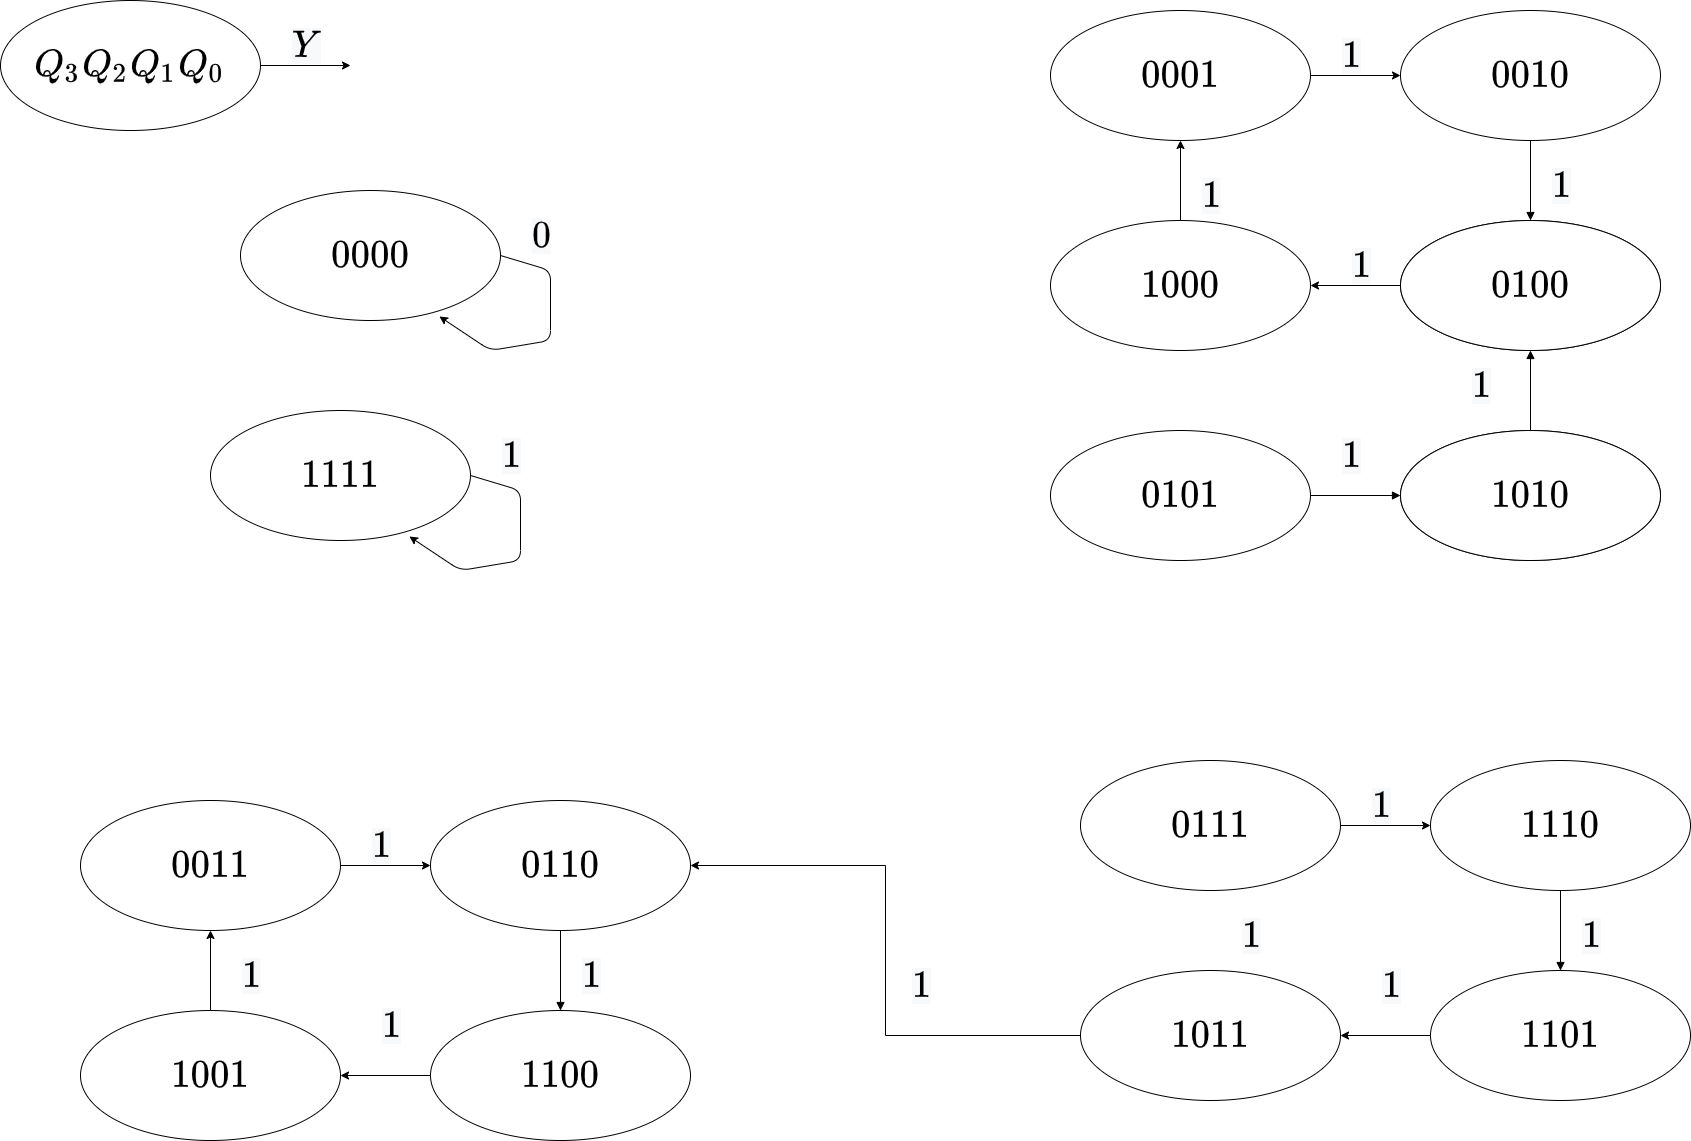
\includegraphics[width=0.45\textwidth]{hw12.png}
    % \caption{#3}
    % \label{#1}
\end{figure}
% Start Here

% End Here

\end{document}